\documentclass[12pt,fleqn]{article}
\renewcommand{\baselinestretch}{1.3}
\usepackage{appendix,hyperref,harvard,amsmath,amssymb,lscape,graphicx,setspace,cancel,amsthm,pgfplots,fullpage}
%\usepackage{amsfonts,latexsym,eurosym}
\bibliographystyle{aer}

%\pdfpagewidth 8.5in
%\pdfpageheight 11in
%\topmargin 0in
%\headheight 0in
%\headsep 0in
%\textheight 9in
%\textwidth 6.5in
%\oddsidemargin 0in
%\evensidemargin 0in
%\headheight 0in
%\headsep 0in

\newcommand{\D}{\displaystyle}
\newcommand{\E}{\begin{eqnarray*}}
\newcommand{\F}{\end{eqnarray*}}
\newcommand{\EE}{\begin{eqnarray}}
\newcommand{\FF}{\end{eqnarray}}
\newcommand{\IZ}{\begin{itemize}}
\newcommand{\ZI}{\end{itemize}}
\newcommand{\EN}{\begin{enumerate}}
\newcommand{\NE}{\end{enumerate}}
\newcommand{\itemc}{\item[$\circ$]}
\newcommand{\IZdash}{\begin{itemize} \renewcommand{\labelitemi}{-}}
\newcommand{\tn}{\textnormal}

%\doublespacing
%\onehalfspacing

\pgfplotsset{height =7cm,compat=1.7,width=7cm,
    standard/.style={
    	unit vector ratio*=1 1 1,
        axis x line=middle,
        axis y line=middle,
        enlarge x limits=0.15,
        enlarge y limits=0.15,
        every axis x label/.style={at={(current axis.right of origin)},anchor=north west},
        every axis y label/.style={at={(current axis.above origin)},anchor=north east}
    }
}
\newcommand{\drawge}{-- (rel axis cs:1,0) -- (rel axis cs:1,1) -- (rel axis cs:0,1) \closedcycle}
\newcommand{\drawle}{-- (rel axis cs:1,1) -- (rel axis cs:1,0) -- (rel axis cs:0,0) \closedcycle}

\usetikzlibrary{patterns}
\usetikzlibrary{arrows}

%%%%%%%%%%%%%%%%%%%%%%%%%%%%%%%%%%%%%%%%%%%%%%%%%%%%%%%%%%%%%%%%%%%%%%%%%%%%%%%%%%%%%%%%%%%%%%%%%%%%
%%%%%%%%%%%%%%%%%%%%%%%%%%%%%%%%%%%%%%%%%%%%%%%%%%%%%%%%%%%%%%%%%%%%%%%%%%%%%%%%%%%%%%%%%%%%%%%%%%%%%

\begin{document}

%\begin{titlepage}
\title{Introduction to Real Business Cycle Modeling}
\author{
%Econ 107: Asymmetric Information\\
Brian Jenkins\\  University of California, Irvine}
\date{\today}

\maketitle
%\begin{abstract}

%\end{abstract}
%\thispagestyle{empty}
%\end{titlepage}

\tableofcontents

\newpage
%%%%%%%%%%%%%%%%%%%%%%%%%%%%%%%%%%%%%%%%%%%%%%%%%%%%%%%%%%%%%%%%%
%%%%%%%%%%%%%%%%%%%%%%%%%%%%%%%%%%%%%%%%%%%%%%%%%%%%%%%%%%%%%%%%%%%%
%\bibliography{EconRef}

\section{Introduction}

Real business cycle (RBC) models are built on the optimizing principles of microeconomics. In these notes, we consider how to solve utility maximization problems in dynamic settings. We first look at a two-period dynamic problem without uncertainty and then we add uncertainty to the two-period framework. Then we make a big jump and consider an infinite-period setting both without and with uncertainty. We'll find that while an infinite-period model with uncertainty may appear significantly more complicated than the deterministic two-period model, the solutions to the optimization problems in each environment are very similar. 

\section{A Two-Period Economy without Labor}

\subsection{The Model without Uncertainty}

A \emph{representative household} lives for two periods. The household receives utility from consuming goods in each period. The \emph{lifetime utility} to the household from consuming $C_0$ in the first period and $C_1$ in the second is denoted by $U(C_0,C_1)$ and is written as:
	\EE
	U(C_0,C_1) & = & u(C_0) + \beta u(C_1),  \label{eqn:two_per_det_utility}
	\FF
where $u(\cdot)$ is the period utility function. We assume that $u(\cdot)$ is strictly increasing and concave. The constant $\beta<1$ reflects the degree to which the household \emph{discounts} utility received in the future relative to utility received in the current period. Figure \ref{fig:two_per_util} depicts a typical period utility function.

	\begin{figure}[t] \caption{\label{fig:two_per_util} Representation of household preferences.}
	\begin{center}

	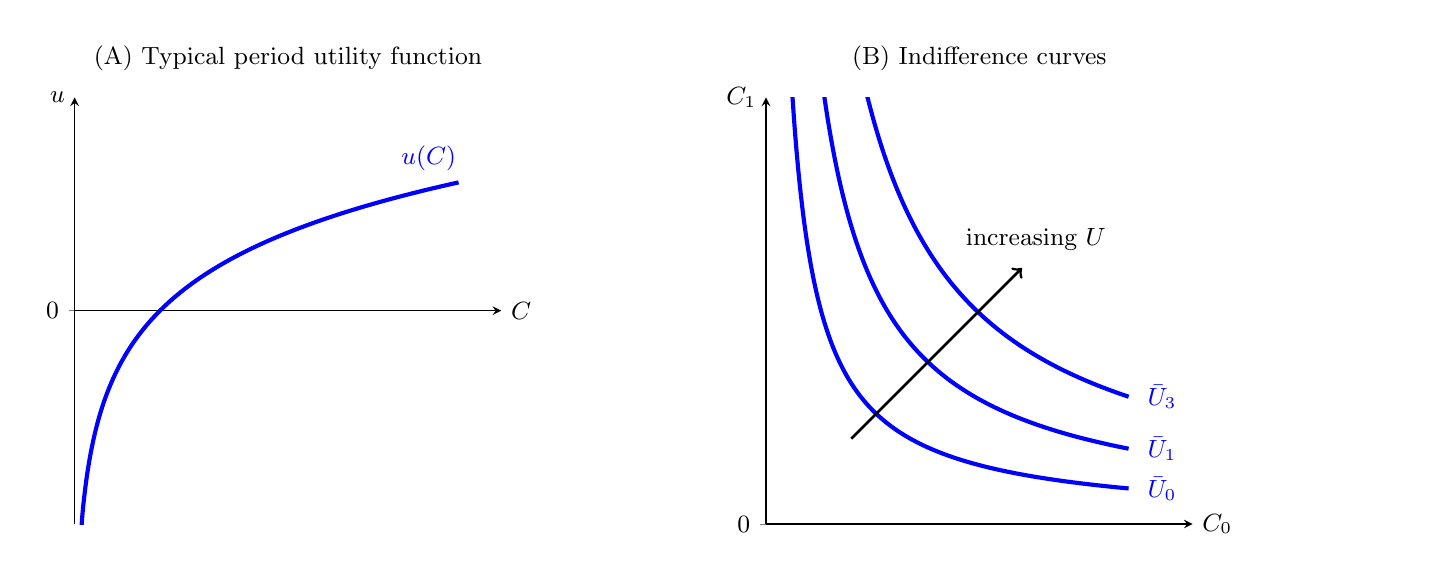
\begin{tikzpicture}
	\matrix{\begin{axis}[standard,%tiny,
    %scale only axis,
    font=\small,
    ytick={0},
    yticklabels={0},
    xtick={0},
    xticklabels={0},
    minor tick num=0,
    axis y line=left,
    axis x line=middle,
    xmin = 0,
    xmax = 5,
    ymin = -2.5,
    ymax = 2.5,
    xlabel style={at=(current axis.right of origin), anchor=west,text width=2.5 cm},
    ylabel style={left},
    xlabel=$C$,ylabel=$u$,
    title={(A) Typical period utility function}
	]
	\addplot[smooth,blue,mark=none,line width = 1.5pt,
	domain=0:4.5,samples=100]
	{ln(x)} node [pos=0.95,inner sep=2pt,label=above:$u(C)$] {};
	%\addplot[smooth,blue,mark=none,line width = 1.5pt,
	%domain=1:4,samples=100]
	%{exp(ln(2)+ln(2.5)-ln(x))} node [pos=0.95,inner sep=2pt,label=right:$\bar{U}^*$] {};
	%\addplot[blue,dotted,mark=,line width = 1pt]
	%coordinates{(0,3) (3,3) (3,0)};
	%\addplot[blue,solid,mark=*,line width = 1pt]
	%coordinates{(3,3)} node[pos=0.5, above, font=\footnotesize, yshift=0pt,xshift = 25pt] {endowment};
	%\addplot[magenta,dotted,mark=,line width = 1pt]
	%coordinates{(2,0) (2,2.5) (0,2.5)};
	%\addplot[magenta,solid,mark=*,line width = 1pt]
	%coordinates{(2,2.5)} ;
	\end{axis}
	&
	\begin{axis}[standard,%tiny,
    %scale only axis,
    font=\small,
    ytick={0},
    yticklabels={0},
    xtick={0},
    xticklabels={0},
    minor tick num=0,
    axis y line=left,
    axis x line=middle,
    xmin = 0,
    xmax = 5,
    ymin = 0,
    ymax = 5,
    xlabel style={at=(current axis.right of origin), anchor=west,text width=2.5 cm},
    ylabel style={left},
    xlabel=$C_0$,ylabel=$C_1$,
    title={(B) Indifference curves}
	]
	%\addplot[smooth,blue,mark=none,line width = 1.5pt,
	%domain=0:4.25,samples=100]
	%{exp(0.25-0.95*ln(x))} node [pos=1,inner sep=2pt,label=right:$\bar{u}_0$] {};
	\addplot[smooth,blue,mark=none,line width = 1.5pt,
	domain=0:4.25,samples=100]
	{exp(.5-0.95*ln(x))} node [pos=1,inner sep=2pt,label=right:$\bar{U}_0$] {};
	\addplot[smooth,blue,mark=none,line width = 1.5pt,
	domain=0:4.25,samples=100]
	{exp(1.25-0.95*ln(x))} node [pos=1,inner sep=2pt,label=right:$\bar{U}_1$] {};
	\addplot[smooth,blue,mark=none,line width = 1.5pt,
	domain=0:4.25,samples=100]
	{exp(1.775-0.95*ln(x))} node [pos=1,inner sep=2pt,label=right:$\bar{U}_3$] {};
	%\addplot[smooth,blue,mark=none,line width = 1.5pt,
	%domain=0:4.25,samples=100]
	%{exp(-0.95*ln(x))} node [pos=1,inner sep=2pt,label=right:$\bar{u}_0$] {};
	
	%\addplot[smooth,blue,mark=none,line width = 1.5pt,
	%domain=1:4,samples=100]
	%{exp(ln(2)+ln(2.5)-ln(x))} node [pos=0.95,inner sep=2pt,label=right:$\bar{U}^*$] {};
	%\addplot[blue,dotted,mark=,line width = 1pt]
	%coordinates{(0,3) (3,3) (3,0)};
	%\addplot[blue,solid,mark=*,line width = 1pt]
	%coordinates{(3,3)} node[pos=0.5, above, font=\footnotesize, yshift=0pt,xshift = 25pt] {endowment};
	%\addplot[magenta,dotted,mark=,line width = 1pt]
	%coordinates{(2,0) (2,2.5) (0,2.5)};
	%\addplot[magenta,solid,mark=*,line width = 1pt]
	%coordinates{(2,2.5)} ;
	\addplot[->,black,mark=none,line width = 1pt]
	coordinates{(1,1) (3,3)} node [pos=1,inner sep=2pt,xshift=5pt,label=above:increasing $U$] {};
	\end{axis}
	\\};
	\end{tikzpicture}
	\end{center}
	\end{figure}
	
The household enters period 0 with $K_0>0$ units of capital which is used to produce $AK_0^{\alpha}$ units of output. Output is allocated between consumption in period 0 and new capital for use in period 1. Capital depreciates at a constant rate $\delta$. The implied budget constraint for period 0 is:
	\EE
	\boxed{C_0 + K_1 = A K_0^{\alpha}  + (1-\delta)K_0}.  \label{eqn:two_per_det_bc0}
	\FF
Note that Equation (\ref{eqn:two_per_det_bc0}) is a representation of the standard requirement that output equals consumption plus investment.\footnote{To see this, define $I_0 = K_1 - (1-\delta)K_0$ and $Y_0 = AK_0^{\alpha}$. Then Equation (\ref{eqn:two_per_det_bc0}) can be written more simply as $Y_0 = C_0 + I_0$.)} For now we're assuming that TFP $A$ is constant. 

In period 1, the household uses its accumulated capital $K_1$ to produce output $AK_1^{\alpha}$. Since period 1 is the final period, the household will consume all of its income \emph{and} accumulated capital so its budget constraint for the second period is:
	\EE
	\boxed{C_1 = A K_1^{\alpha}  + (1-\delta)K_1}.  \label{eqn:two_per_det_bc1}
	\FF
Given the household's initial capital holding $K_0>0$, Equations (\ref{eqn:two_per_det_bc0}) and (\ref{eqn:two_per_det_bc1}) constrain the feasible set of combinations of the household's consumption in the two periods.

The household's objective is to choose consumption in each period and a level of saving to maximize its lifetime utility (\ref{eqn:two_per_det_utility}) subject to the two budget constraints (\ref{eqn:two_per_det_bc0}) and (\ref{eqn:two_per_det_bc1}). We can express the optimization problem concisely as:
	\EE
	&&\max_{C_0,C_1,K_1} \; u(C_0) + \beta u(C_1)\\\nonumber\\
	&& \; \; \; \;  \; \; \; \; \tn{s.t.} \; \; \; \; C_0 + K_1 = A K_0^{\alpha}  + (1-\delta)K_0\nonumber\\
	&&\; \; \; \; \; \; \; \; \; \; \; \; \; \; \; \; \; C_1 = A K_1^{\alpha}  + (1-\delta)K_1.\nonumber
	\FF
To solve this constrained optimization problem, we will use the constraints to eliminate $C_0$ and $C_1$ from the problem so that we are left with an unconstrained optimization problem.\footnote{Alternatively, we could certainly use the method of Lagrange multipliers.} After making the substitutions, we obtain the simplified representation of the problem:
	\EE
	\max_{K_1} \; u\Big( A K_0^{\alpha}  + (1-\delta)K_0 - K_1 \Big) + \beta u\Big( A K_1^{\alpha}  + (1-\delta)K_1 \Big)
	\FF
Next we solve the problem by setting derivative of the objective function with with respect to $K_1$ equal to zero:
	\EE
	&& u'\Big( A K_0^{\alpha}  + (1-\delta)K_0 - K_1 \Big) \nonumber \\
	&& \; \; \; \; \; \; \; \; \; \; \; \; = \left( \alpha AK_1^{\alpha-1} + 1-\delta\right) \beta u'\Big( A K_1^{\alpha}  + (1-\delta)K_1 \Big) \label{eqn:two_per_det_k1_foc},
	\FF
where $u'(\cdot)$ denotes the period marginal utility of consumption. Equation (\ref{eqn:two_per_det_k1_foc}) is the \emph{first-order condition} for the optimal choice of $K_1$. Notice that the arguments of $u'(\cdot)$ in Equation (\ref{eqn:two_per_det_k1_foc}) are still equal to $C_0$ and $C_1$. This means that we can rewrite the first-order condition for $S_1$ in terms of consumption:
	\EE
	\boxed{u'(C_0) = \beta \left( \alpha AK_1^{\alpha-1} + 1-\delta\right) u'(C_1)} \label{eqn:two_per_det_euler}
	\FF
Equation (\ref{eqn:two_per_det_euler}) is called the household's \emph{consumption Euler equation}. The consumption Euler equation -- or just Euler equation, for short -- indicates that the optimal choice of consumption in period 0 depends on consumption in period 1 and gross return on capital: $1 + \alpha AK_1^{\alpha-1} - \delta$. The equilibrium values of $C_0$, $C_1$, and $K_1$ are fully characterized by Equations (\ref{eqn:two_per_det_bc0}), (\ref{eqn:two_per_det_bc1}), and (\ref{eqn:two_per_det_euler}) given some initial value of capital $K_0>0$.

\subsection{A Specific Example}

In general, the system of equations described by Equations (\ref{eqn:two_per_det_bc0}), (\ref{eqn:two_per_det_bc1}), and (\ref{eqn:two_per_det_euler}) cannot be solved analytically; i.e., with pencil and paper. However, if we assume log utility and full capital depreciation, then the equilibrium \emph{does} admit an analytical solution. Specifically, suppose $u(C) = \log C$ and $\delta = 1$. Then the equilibrium conditions can be rewritten as:
	\EE
	\frac{1}{C_0} & = & \frac{\beta\alpha K_1^{\alpha - 1}}{C_1}\\
	C_0 & = & AK_0^{\alpha} - K_1\\
	C_1 & = & AK_1^{\alpha},
	\FF
which implies:
	\EE
	K_1 & = & \alpha \beta AK_0^{\alpha}\\
	C_0 & = & (1-\alpha \beta)A K_0^{\alpha}\\
	C_1 & = & A K_1^{\alpha}
	\FF

\subsection{The Model with Random TFP}


Until now we've been assuming that TFP is constant across periods. Now, suppose that TFP takes the values $A_0$ and $A_1$ in each period. Furthermore, suppose that as of the time that the household solves its optimization problem in period 0, the value of $A_0$ is known but the value of $A_1$ is not known. If the value of $A_1$ is uncertain, then the household can't know for sure what its consumption in period 1 will be and so instead of simply maximizing its lifetime utility, the household will have to maximize its \emph{expected} lifetime utility.


To make things a little easier, suppose that the household has log utility. Therefore, we write the household's maximization problem given uncertainty over $A_1$ as:
	\EE
	&&\max_{C_0,C_1,K_1} \; \log(C_0) + \beta E_0\log (C_1)\\\nonumber\\
	&& \; \; \; \;  \; \; \; \; \tn{s.t.} \; \; \; \; C_0 + K_1 = A_0 K_0^{\alpha}  + (1-\delta)K_0\nonumber\\
	&&\; \; \; \; \; \; \; \; \; \; \; \; \; \; \; \; \; C_1 = A_1 K_1^{\alpha}  + (1-\delta)K_1,\nonumber
	\FF 
where $E_0u(C_1)$ denotes the \emph{expectation of the flow of utility from $C_1$ given all information available at date 0}. The household maximizes is \emph{expected utility}. Notice that the constraints on $C_0$ and $C_1$ are the same as the case without uncertainty except now we have to account for the time-dependent values of TFP.

We solve the problem with uncertainty in the same way that we solved the problem without uncertainty: use the constraints to eliminate $C_0$ and $C_1$ from the problem and find the first-order condition with respect to $K_1$. After eliminating $C_0$ and $C_1$, the problem becomes:
	\EE
	\max_{K_1} \; \log \Big( A K_0^{\alpha}  + (1-\delta)K_0 - K_1 \Big) + \beta E_0 \log \Big( A K_1^{\alpha}  + (1-\delta)K_1 \Big). \label{eqn:opt_prob_simplified2}
	\FF
Next we solve the problem by differentiating Equation (\ref{eqn:opt_prob_simplified2}) with respect to $K_1$ and setting that equal to zero to obtain:
	\EE
	 - \frac{1}{A K_0^{\alpha}  +  (1-\delta)K_0 - K_1}  +  \beta E_0 \left[\frac{ \alpha A_1K_1^{\alpha-1} + 1-\delta}{A_1 K_1^{\alpha}  + (1-\delta)K_1}\right] & = & 0 \label{eqn:two_per_stoch_k1_foc},
	\FF
Notice that in order to differentiate the second term in Equation (\ref{eqn:opt_prob_simplified2}) with respect to $K_1$, we simply passed the the derivative operation through the expectation.\footnote{It's tempting to try to simplify the term in square brackets further writing it as a quotient of two expectations, but that's not a legal move:
	\EE
	E_0 \left[  \frac{\alpha A_1 K_1^{\alpha-1}  + 1-\delta}{ A_1 K_1^{\alpha}  + (1-\delta)K_1}\right] & \ne   \D   \frac{\D E_0 \left[\alpha A_1 K_1^{\alpha-1}  + 1-\delta\right]}{ \D E_0 \left[ A_1 K_1^{\alpha}  + (1-\delta)K_1\right] }.
	\FF}
As before, we can use the budget constraints to simplify the first-order condition for $K_1$. Then given $K_0>0$, the equilibrium values of $C_0$, $C_1$, and $K_1$ are characterized by the following three conditions:
	\EE
	\frac{1}{C_0} & = &  \beta E_0 \left[ \frac{\alpha A_1K_1^{\alpha-1} + 1-\delta}{C_1}\right]\\
	C_0 + K_1 & = &  A_0 K_0^{\alpha}  + (1-\delta)K_0\\
	C_1 & = &  A_1 K_1^{\alpha}  + (1-\delta)K_1
	\FF
Notice that these are identical to the equilibrium conditions for the two period model without uncertainty except for the expectation in the Euler equation. Apparently adding uncertainty about TFP does little to change the appearance of the equilibrium conditions. Of course, the model is incomplete without a specification for how $A_1$ is determined, but we'll confront that later.

\section{An Infinite-Horizon Economy without Labor}

\subsection{The Model without Uncertainty}

Suppose now that a \emph{representative household} lives for an infinite number of periods. As in the two-period model, the household receives utility from consuming goods in each period. The lifetime utility to the household from an infinite consumption stream $C_0, C_1, C_2, \ldots$ is denoted by $U_0$ and is written as:
	\EE
	U & = & \log (C_0) + \beta  \log (C_1) + \beta^2 \log (C_2)  + \beta^3 \log (C_3)+ \cdots\\
	& = & \sum_{t = 0}^{\infty} \beta^t \log (C_t),  \label{eqn:infinite_per_det_utility}
	\FF
As before, the constant $\beta<1$ reflects the degree to which the household \emph{discounts} utility received in the future.
	
The household enters period 0 with $K_0>0$ units of capital and faces the following sequence of budget constraints:
\EE
C_0 + K_1 & = & A K_0^{\alpha}  + (1-\delta)K_0 \\
C_1 + K_2 & = & A K_1^{\alpha}  + (1-\delta)K_1 \\
C_2 + K_3 & = & A K_2^{\alpha}  + (1-\delta)K_2 \\
%\vdots \; \; \; \; \; \; & \vdots & \; \; \; \; \; \; \; \; \; \; \; \; \; \;  \vdots 
& \vdots & 
\FF
Note that TFP $A$ is assumed to be constant across all periods. We can express the sequence of constraints more concisely as 
\EE
C_t + K_{t+1} & = & A K_{t}^{\alpha}  + (1-\delta)K_t, \; \; \; \; \; \text{for } t = 0,1,2,3\ldots \label{eqn:infinite_per_det_bc}
\FF

Now we can use Equation (\ref{eqn:infinite_per_det_bc}) to express the household's utility in terms of only capital in each period:
	\EE
	U 	& = & \sum_{t = 0}^{\infty} \beta^t \log (C_t) \\
		& = & \sum_{t = 0}^{\infty} \beta^t \log \Big(A K_{t}^{\alpha}  + (1-\delta)K_t - K_{t+1}\Big) \\
		& = & \log \Big(A K_{0}^{\alpha}  + (1-\delta)K_0 - K_{1}\Big) + \beta \log \Big(A K_{1}^{\alpha}  + (1-\delta)K_1 - K_{2}\Big) \nonumber\\
		& & \; \; \; \; \; \; \; + \, \beta^2 \log \Big(A K_{2}^{\alpha}  + (1-\delta)K_2 - K_{3}\Big) \nonumber\\
		& & \; \; \; \; \; \; \; \; \; \; \; \; \; \; + \, \beta^3 \log \Big(A K_{3}^{\alpha}  + (1-\delta)K_3 - K_{4}\Big) + \cdots \label{eqn:infinite_per_det_utility_subs}
	\FF


The household's maximization problem is to choose:
	\EE
	&&\max_{C_0,C_1,C_2,\ldots,K_1,K_2,K_3,\ldots} \; \sum_{t=0}^{\infty}\beta^t\log (C_t) \\\nonumber\\
	&& \; \; \; \;  \; \; \; \; \tn{s.t.} \; \; \; \; C_t + K_{t+1} = A K_{t}^{\alpha}  + (1-\delta)K_t\nonumber
	\FF 
Just like we did with the two period model, we can substitute the constraint into the utility function to eliminate consumption from the maximization problem:
	\EE
	&&\max_{K_1,K_2,K_3,\ldots} \; \sum_{t=0}^{\infty}\beta^t\log \Big(A K_{t}^{\alpha}  + (1-\delta)K_t - K_{t+1}\Big) 
	\FF 
The problem has an infinite number of first-order conditions: one for $K_1$, $K_2$, $K_3$, $K_4$, and so on. Looking at Equation (\ref{eqn:infinite_per_det_utility_subs}), the first-order condition for $K_1$ is apparently:
	\EE
	-\frac{1}{A K_{0}^{\alpha}  + (1-\delta)K_0 - K_{1}} + \beta\frac{\alpha A K_{1}^{\alpha-1}  + 1-\delta}{A K_{1}^{\alpha}  + (1-\delta)K_1 - K_{2}} & = & 0,
	\FF
which implies:
	\EE
	\frac{1}{C_0} & = & \frac{\beta\left(\alpha A K_1^{\alpha - 1} + 1 - \delta\right)}{C_1}
	\FF
And the first order condition for $K_2$ is evidently:
	\EE
	-\beta\frac{1}{A K_{1}^{\alpha}  + (1-\delta)K_1 - K_{2}} + \beta^2\frac{\alpha A K_{2}^{\alpha-1}  + 1-\delta}{A K_{2}^{\alpha}  + (1-\delta)K_2 - K_{3}} & = & 0,
	\FF
which implies:
	\EE
	\frac{1}{C_1} & = & \frac{\beta\left(\alpha A K_2^{\alpha - 1} + 1 - \delta\right)}{C_2}
	\FF
Evidently there is a pattern. The first-order condition with respect to $K_{t+1}$ is:
	\EE
	-\frac{1}{A K_{t}^{\alpha}  + (1-\delta)K_t - K_{t+1}} + \beta\frac{\alpha A K_{t+1}^{\alpha-1}  + 1-\delta}{A K_{t+1}^{\alpha}  + (1-\delta)K_1 - K_{t+2}} & = & 0,
	\FF
which implies the following general Euler equation linking any two periods $t$ and $t+1$:
	\EE
	\boxed{\frac{1}{C_t} = \frac{\beta\left(\alpha A K_{t+1}^{\alpha - 1} + 1 - \delta\right)}{C_{t+1}}} \label{eqn:infinite_per_det_euler}
	\FF
Given $K_0>0$, the equilibrium sequences of consumption $C_0, C_1, C_2, \ldots$ and capital $K_1, K_2, K_3, \ldots$ are characterized by the Euler equation (\ref{eqn:infinite_per_det_euler}) and the budget constraint (\ref{eqn:infinite_per_det_bc}).
	
	
	
\subsection{The Infinite-Horizon Model with Random TFP}


Now, suppose that TFP in period 0 is known to the household but that TFP for subsequent periods is stochastic. That is, $A_0$ is known to the household but $A_1, A_2, A_3, \ldots$ are not. Since the future values of TFP are uncertain, the household can only maximize its \emph{expected} lifetime utility given what it knows about the economy as of date 0.

Specifically, \emph{each period} the household information available at the time and chooses current consumption $C_t$ and capital for next period $K_{t+1}$. This means that at date 0, the household chooses $C_0$ and $K_1$, but can't choose $C_1$ yet because TFP and therefore output for period 1 is known yet. So in period 0, the household solves:
	\EE
	&&\max_{C_0,K_1} \; E_0\sum_{t=0}^{\infty}\beta^t\log (C_t) \\\nonumber\\
	&& \; \; \; \;  \; \; \; \; \tn{s.t.} \; \; \; \; C_t + K_{t+1} = A_t K_{t}^{\alpha}  + (1-\delta)K_t\nonumber
	\FF 
And just like we did with the two period model, we can substitute the constraint into the utility function to eliminate consumption from the maximization problem:
	\EE
	&&\max_{K_1} \; E_0\sum_{t=0}^{\infty}\beta^t\log \Big(A_t K_{t}^{\alpha}  + (1-\delta)K_t - K_{t+1}\Big) 
	\FF
Now note that even though the function to be maximized is an infinite sum, only the first two terms of the sum contain $K_1$:
	\EE
	&& E_0\sum_{t=0}^{\infty}\beta^t\log \Big(A_t K_{t}^{\alpha}  + (1-\delta)K_t - K_{t+1}\Big)   \\
	&& \; \; \; \; \; \; \; \; \; \; \; \; \; \; \; = \,  \log\Big(A_0 K_0^{\alpha} + (1-\delta)K_0 - K_1\Big) \nonumber \\
	&& \; \; \; \; \; \; \; \; \; \; \; \; \; \; \; \; \; \; \; \; + \, \beta E_0 \log\Big(A_1 K_1^{\alpha} + (1-\delta)K_1 - K_2\Big)\nonumber \\
	&  & \; \; \; \; \; \; \; \; \; \; \; \; \; \; \; \; \; \; \; \; \; \; \; \; \; + \, \left[\text{terms independent of $K_1$}\right]
	\FF
Therefore, the first-order condition with respect to $K_1$ is:
	\EE
    -\frac{1}{\underbrace{A_0 K_{0}^{\alpha}  + (1-\delta)K_0 - K_{1}}_{C_0}} + \beta E_0 \bigg[\frac{\alpha A_1 K_1^{\alpha - 1} + 1 - \delta}{\underbrace{A_{1} K_{1}^{\alpha}  + (1-\delta)K_{1} - K_{2}}_{C_1}}\bigg] & = & 0,
    \FF
which can be written more concisely as:
	\EE
	\frac{1}{C_0} & = & \beta E_0 \left[\frac{\alpha A_{1}K_1^{\alpha - 1} + 1 - \delta}{C_1}\right]
	\FF
This expression should look familiar given the what has been derived earlier.

The household solves similar problems in periods $1, 2, 3, \ldots$ and the following general Euler equation characterizes the solution to the household's optimization problem in period each period $t$:
	\EE
	\boxed{\frac{1}{C_t} = \beta E_t \left[\frac{\alpha A K_{t+1}^{\alpha - 1} + 1 - \delta}{C_{t+1}}\right]} \label{eqn:infinite_per_stoch_euler}
	\FF
Given $K_0>0$, the equilibrium sequences of consumption $C_0, C_1, C_2, \ldots$ and capital $K_1, K_2, K_3, \ldots$ are characterized by the Euler equation (\ref{eqn:infinite_per_stoch_euler}) and the budget constraint:
\EE
\boxed{C_t + K_{t+1} = A K_{t}^{\alpha}  + (1-\delta)K_t} \label{eqn:infinite_per_stoch_bc}
\FF




\end{document}

%%%%%%%%%%%%%%%%%%%%%%%%%%%%%%%%%%
%%%%%%%%%%%%%%%%%%%%%%%%%%%%%%%%%%
%%% Example table %%%%%%%%%%%%%%%%
%%%%%%%%%%%%%%%%%%%%%%%%%%%%%%%%%%
%%%%%%%%%%%%%%%%%%%%%%%%%%%%%%%%%%


\begin{landscape}
\begin{table}[] \caption{\label{} Optimal monetary policy from Schmitt-Groh\'{e} and Uribe 2007}

\
\begin{tabular}{llllllll} \hline
 & $\alpha_{\pi}$ & $\alpha_y$ & $\alpha_R$ &  Conditional welfare & Unconditional welfare & $\sigma_{\pi}$ & $\sigma_{R}$ \\
 & & & & cost ($\lambda^c \times 100$) & cost ($\lambda^c \times 100$)\\ \hline
 \textbf{A. The cashless economy} {\rule[0mm]{0mm}{5mm}}\\
 Ramsey Policy & - & - & - & ~0 & 0 &0.01 &  0.27 \\
 Optimized Rules \\
 Contemporaneous ($i=0$)\\
 {\rule[0mm]{1.0mm}{0mm}} Smoothing & 3 & 0.01 & 0.84 & ~0.000 & 0.000 & 0.04 &  0.29 \\
 {\rule[0mm]{1.0mm}{0mm}} No Smoothing & 3 & 0.00 & - & ~0.000 & 0.001 & 0.14 &  0.42 \\
 Backward ($i=1$) & 3 & 0.03 & 1.71 & ~0.001 & 0.001 & 0.10 &  0.23 \\
 Forward ($i=-1$) & 3 & 0.07 & 1.58 & ~0.002 & 0.003 & 0.19 & 0.27 \\
 Nonoptimized rules\\
 Taylor rule ($i=0$) & 1.5 & 0.5 & - & ~0.451 & 0.522 & 3.19 & 3.08\\
 Simple Taylor rule & 1.5 & - & - & ~0.014 & 0.019 & 0.58 & 0.87\\
 \\
 \textbf{B. The monetary economy} {\rule[0mm]{0mm}{5mm}}\\
 Ramsey Policy & - & - & - & ~0 & 0 &0.01 & 0.27 \\
 Optimized Rules \\
 Contemporaneous ($i=0$)\\
 {\rule[0mm]{1.0mm}{0mm}} Smoothing & 3 & 0.01 & 0.80 & ~0.000 & 0.000 & 0.04 & 0.29 \\
 {\rule[0mm]{1.0mm}{0mm}} No Smoothing & 3 & 0.00 & - & ~0.001 & 0.001 & 0.14 & 0.41 \\
 Nonoptimized rules\\
 Taylor rule ($i=0$) & 1.5 & 0.5 & - & ~0.598 & 0.709 & 3.93 & 3.76\\
 {\rule[3mm]{0mm}{0mm}}Simple Taylor rule & 1.5 & - & - & ~0.011 & 0.015 & 0.56 & 0.85\\\hline
 \end{tabular}
\end{table}

\end{landscape}







%%%%%%%%%%%%%%%%%%%%%%%%%%%%%%%%%%
%%%%%%%%%%%%%%%%%%%%%%%%%%%%%%%%%%
%%% Example figure and graphic %%%
%%%%%%%%%%%%%%%%%%%%%%%%%%%%%%%%%%
%%%%%%%%%%%%%%%%%%%%%%%%%%%%%%%%%%


\begin{figure}[h] \caption{\label{} The welfare cost of responding to output: varying $\alpha_y$ holding $\alpha_{\pi} =3$ and $\alpha_R = 0$.}
\includegraphics[height = 10cm]{fig1.png}
\end{figure}

